The objective of this study is to determine whether a demand forecaster trained
end-to-end to minimise an \emph{asymmetric operational cost} can outperform both
a symmetric-loss model and the real operational forecast of the Israeli system
operator, under the cost asymmetries characteristic of electricity procurement.
This section describes the material and procedures used to answer that question:
the dataset (Section~\ref{sec:dataset}), the neural architecture and the three
training objectives we compare, and the protocol under which they are evaluated
(Section~\ref{sec:model-training}).

\subsection{Dataset}
\label{sec:dataset}
In this section we describe the dataset we used for our experiments. 
The dataset consists of both electricity consumption and weather data, collected from various sources. 
The electricity consumption data was obtained from the Israeli electricity system operator Noga~(\cite{noga}), 
while the weather data was sourced from a nearby meteorological station~(\cite{ims}).
Electricity consumption data includes hourly readings of power usage.
Crucially, it also includes the \emph{real day-ahead forecasts} published by Noga as part of the
market clearing process.  These are the actual forecasts used by the system operator in the
day-ahead market, not post-hoc reconstructions.  Their inclusion in our dataset
provides two important opportunities: (i)~we can directly compare the performance
of our learned models against the operational forecasts actually used in the market,
serving as a strong real-world baseline; and (ii)~we can analyze the
distribution of real-world prediction errors produced by an experienced operator,
which motivates and contextualizes the cost asymmetries studied in this paper.
The weather data includes temperature, humidity, and wind speed measurements taken every three hours in the three major cities of Israel: Tel Aviv, Jerusalem, and Haifa.
% Table~\ref{tab:electricity-fields} summarizes the fields present in the electricity consumption data,
% and Table~\ref{tab:weather-fields} summarizes the fields present in the weather data. 
% The dataset covers the period from March 2023 to February 2026, 
% providing a comprehensive view of electricity consumption patterns 
% and their relationship with weather conditions over the course of almost three years.

% \begin{table}[ht]
%     \centering
%     \begin{tabular}{ll}
%         \hline
%         \textbf{Field} & \textbf{Description} \\
%         \hline
%         \texttt{date} & Calendar date (DD-MM-YYYY). \\
%         \texttt{total\_demand} & Total daily electricity demand (MWh). \\
%         \texttt{total\_day\_ahead\_forecast} & Operator's day-ahead forecast (MWh). \\
%         \hline
%     \end{tabular}
%     \caption{Electricity consumption data fields (daily aggregated from hourly source data).}
%     \label{tab:electricity-fields}
% \end{table}

% \begin{table}[ht]
%     \centering
%     \begin{tabular}{ll}
%         \hline
%         \textbf{Field} & \textbf{Description} \\
%         \hline
%         \texttt{temperature\_Haifa} & Daily mean temperature, Haifa ($^\circ$C). \\
%         \texttt{temperature\_Jerusalem} & Daily mean temperature, Jerusalem ($^\circ$C). \\
%         \texttt{temperature\_Tel\_Aviv} & Daily mean temperature, Tel~Aviv ($^\circ$C). \\
%         \hline
%     \end{tabular}
%     \caption{Weather data fields (daily means aggregated from tri-hourly station observations).}
%     \label{tab:weather-fields}
% \end{table}

\subsection{Data Analysis}
To better understand the dataset, we performed an exploratory data analysis (EDA) to identify patterns and relationships between the electricity consumption and weather data.
Figure~\ref{fig:daily-demand} shows the daily electricity consumption over the course of the dataset alongside the daily average temperature in Tel Aviv.

\begin{figure}[ht]
    \centering
    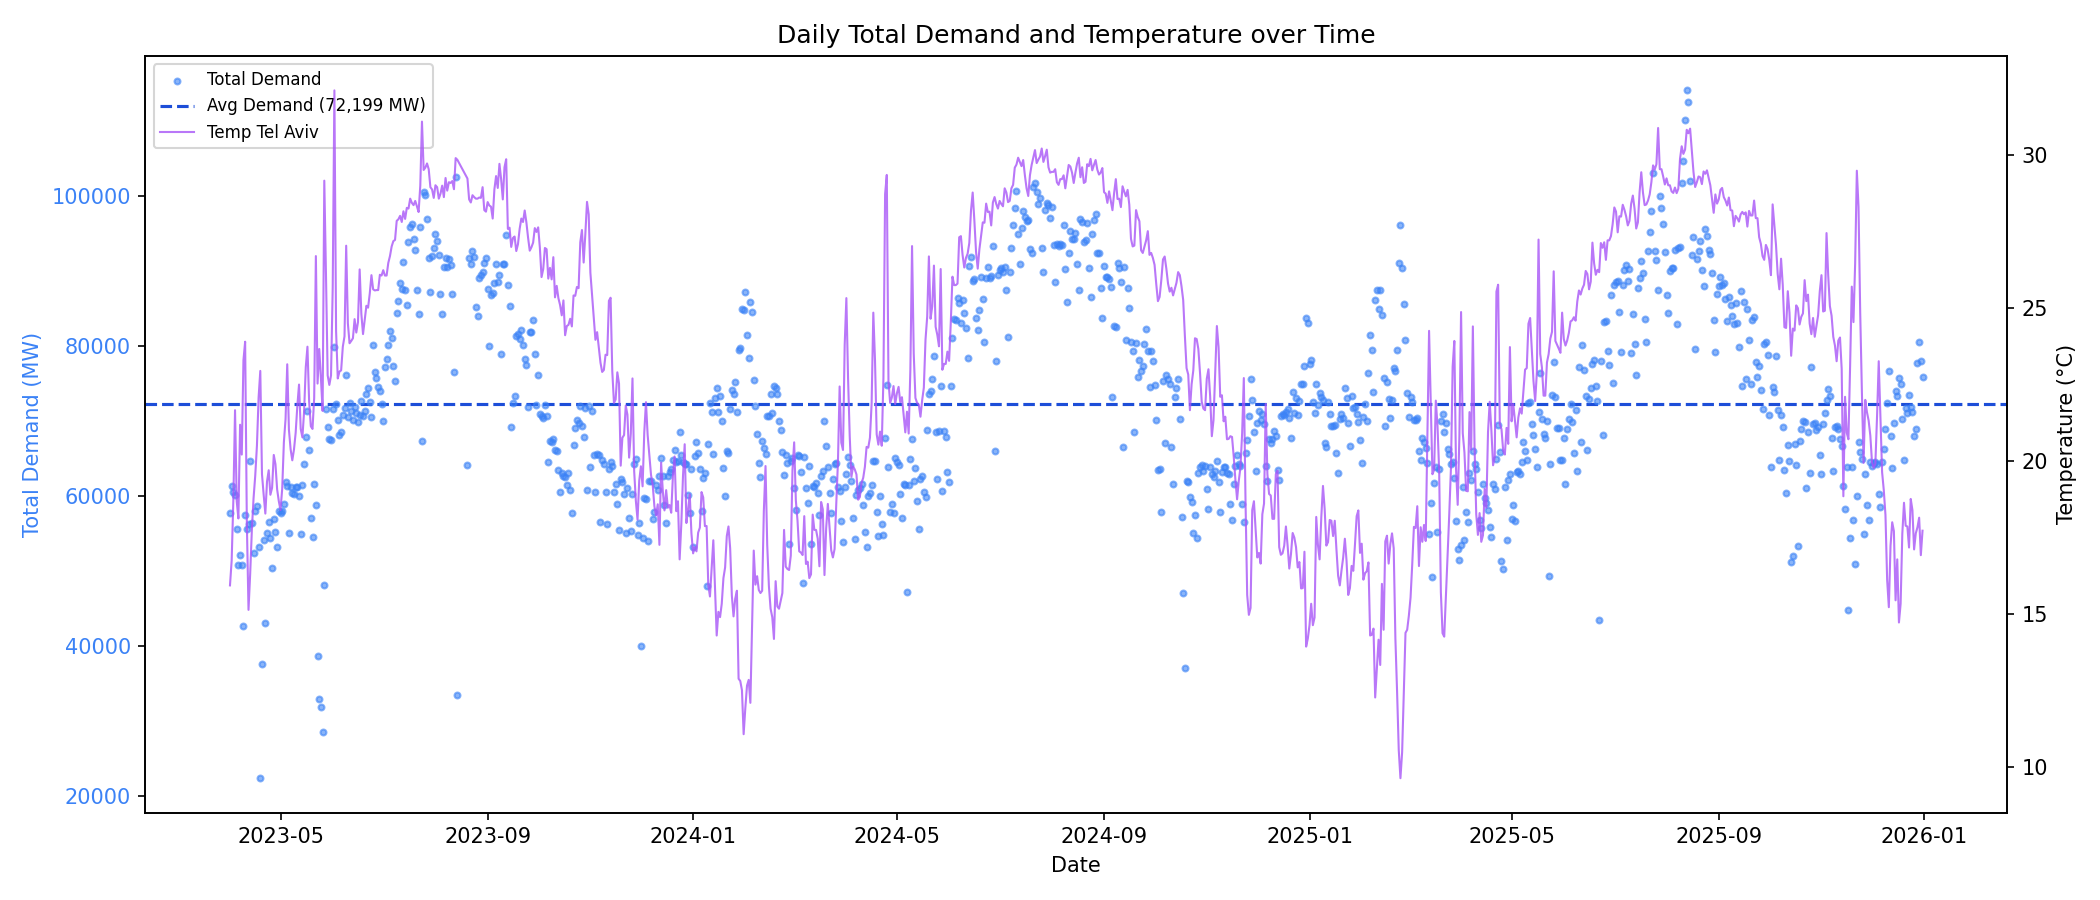
\includegraphics[width=\textwidth]{plot/daily_demand_by_time.png}
    \caption{Daily electricity consumption (MWh) over the dataset period
    (March~2023--February~2026).  Clear seasonal patterns are visible, with
    a summer peak (July--August) driven by air-conditioning loads and a secondary
    winter peak (January--February) driven by heating.}
    \label{fig:daily-demand}
\end{figure}

Figure~\ref{fig:daily-demand-vs-temp} shows the relationship between daily electricity consumption and the daily average temperature in Tel Aviv.

\begin{figure}[ht]
    \centering
    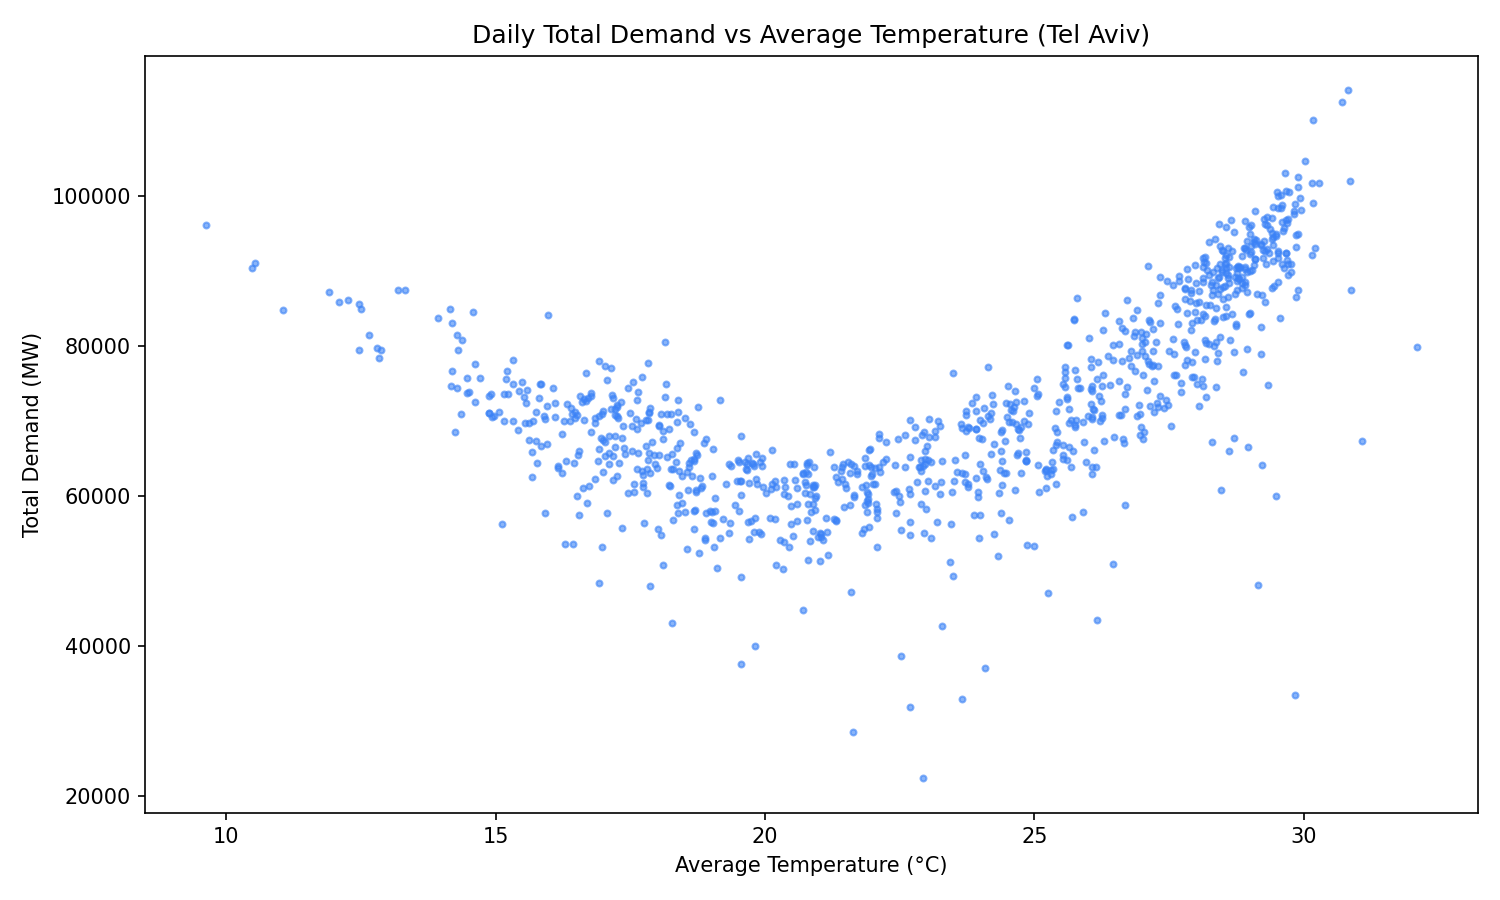
\includegraphics[width=\textwidth]{plot/daily_demand_vs_avg_temp_Tel_Aviv.png}
    \caption{Daily electricity consumption vs.\ daily mean temperature in
    Tel~Aviv.  The characteristic U-shaped relationship is visible, with
    high demand at both high temperatures (cooling loads) and low temperatures
    (heating loads).  The balance-point temperature is approximately
    20\,$^\circ$C.}
    \label{fig:daily-demand-vs-temp}
\end{figure}

% Figure~\ref{fig:daily-demand-vs-forecast-time} depicts the relationship between daily electricity consumption and the operator's day-ahead forecast over time.

% \begin{figure}[ht]
%     \centering
%     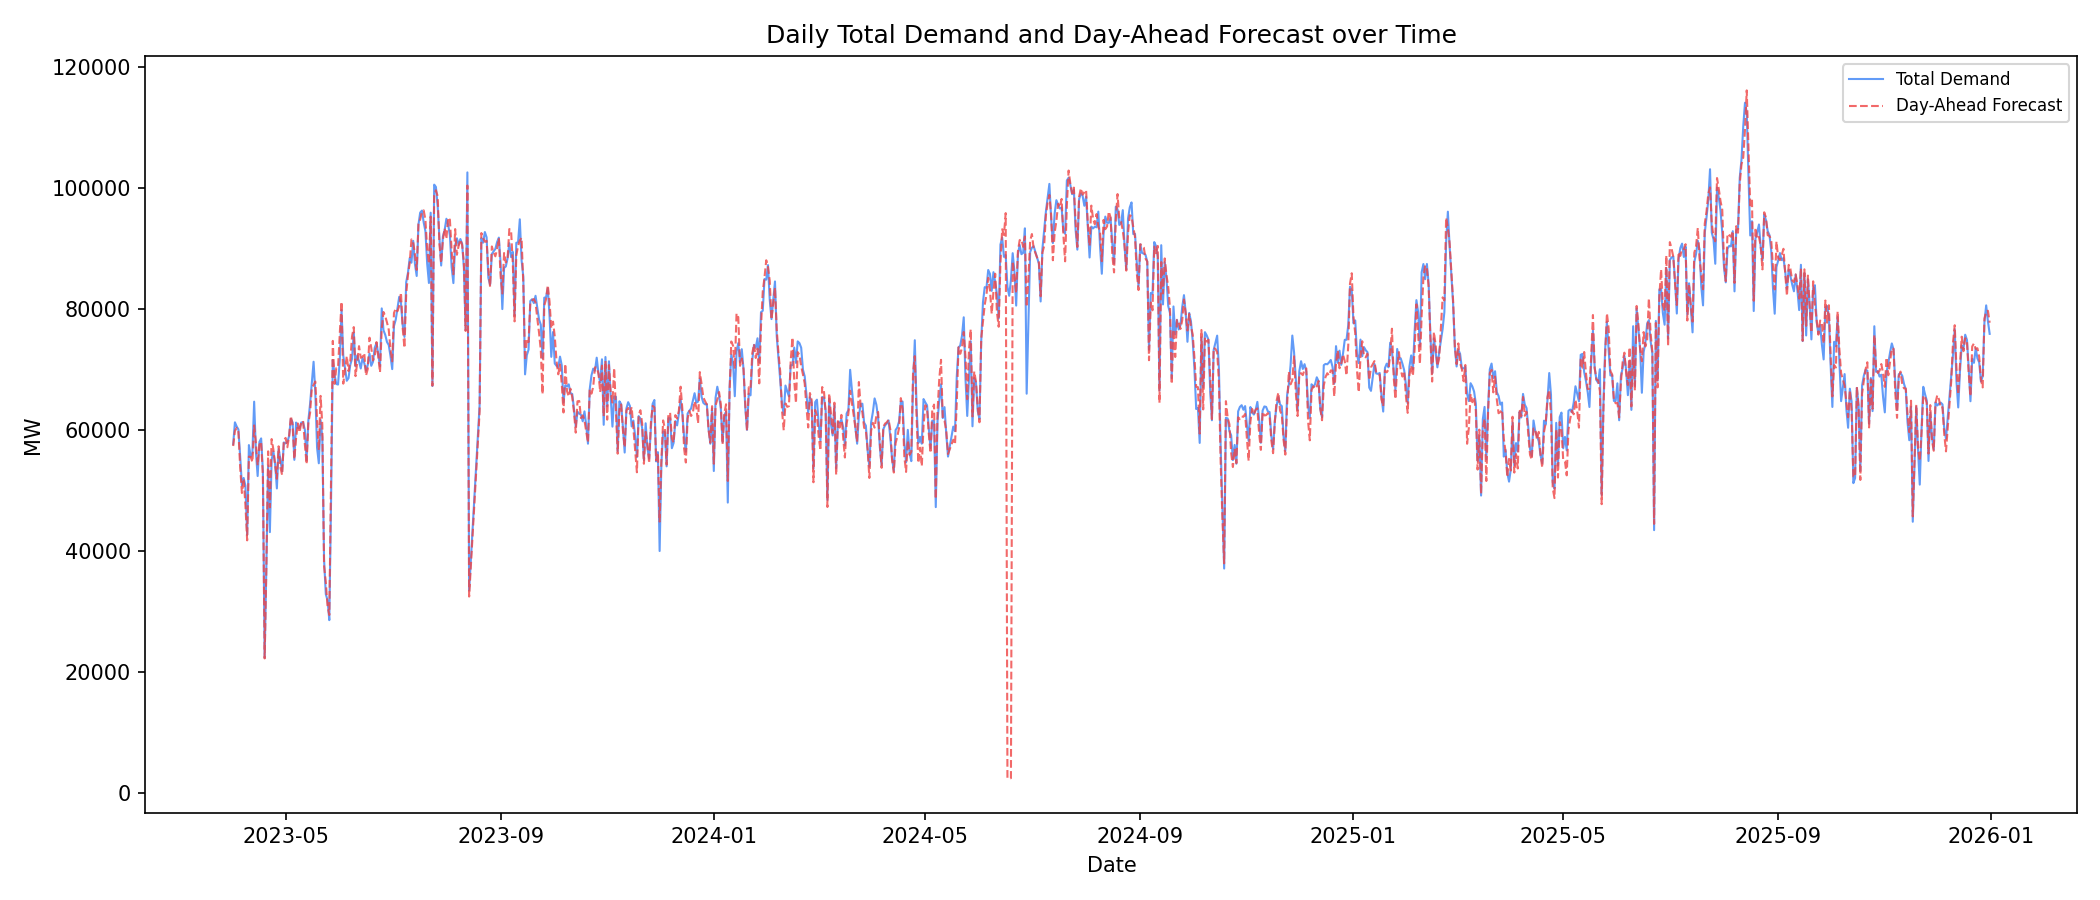
\includegraphics[width=\textwidth]{plot/daily_demand_vs_forecast_time.png}
%     \caption{Daily electricity consumption (solid blue) vs.\ operator day-ahead
%     forecast (dashed orange) over time.  The forecast tracks actual demand
%     closely, with visible errors during demand spikes.}
%     \label{fig:daily-demand-vs-forecast-time}
% \end{figure}

Figure~\ref{fig:demand-vs-forecast-kde} shows the KDE histogram of the forecast error, i.e., the difference between the actual demand and the day-ahead forecast.

\begin{figure}[ht]
    \centering
    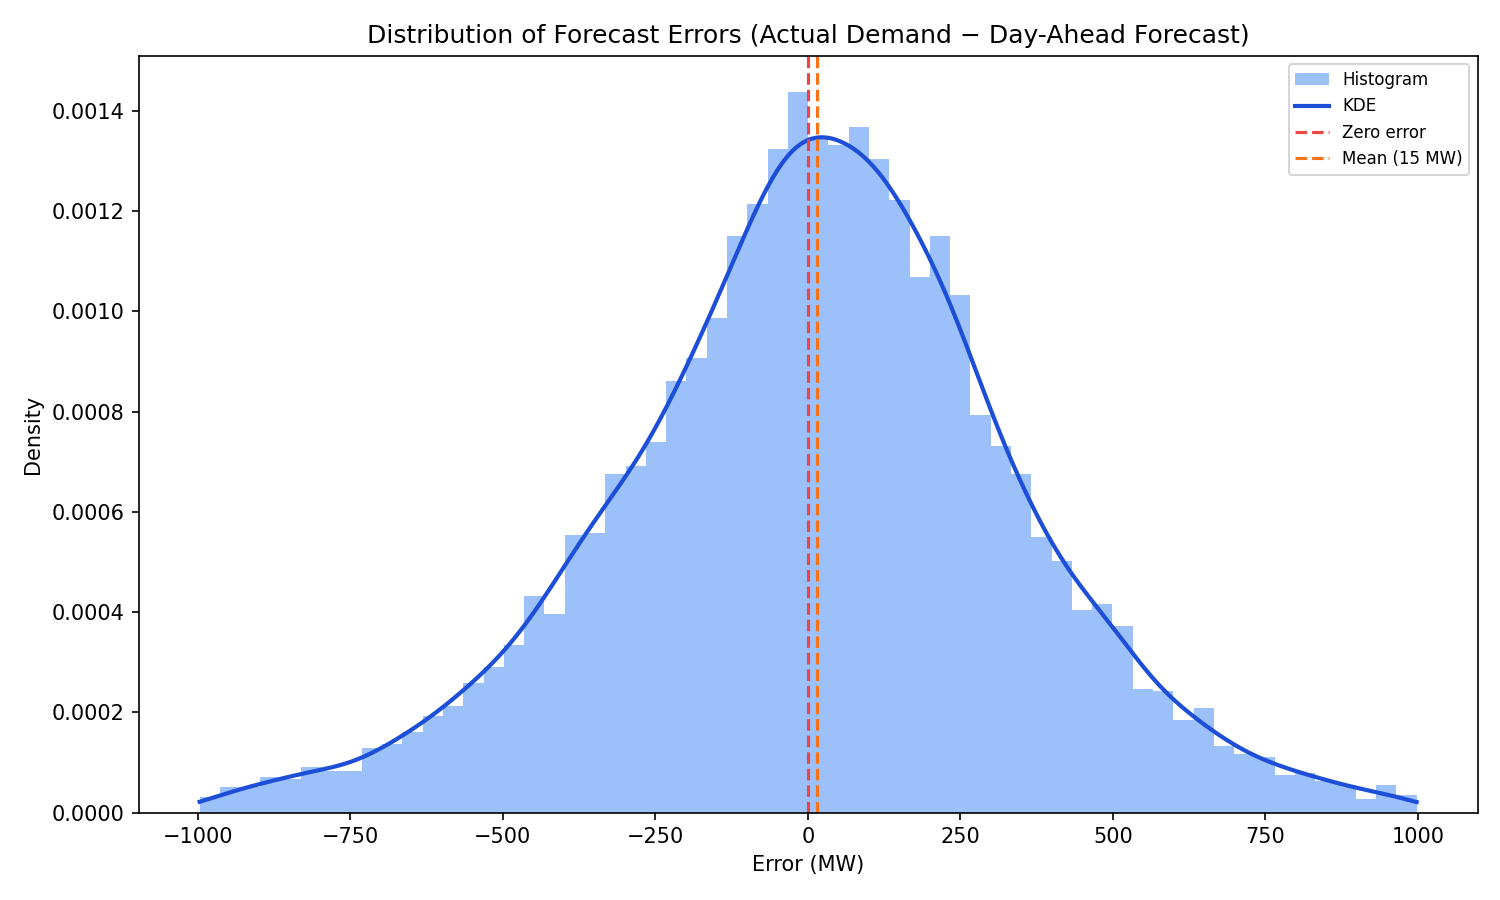
\includegraphics[width=\textwidth]{plot/demand_vs_forecast_kde_histogram.png}
    \caption{KDE histogram of the forecast error (actual demand minus
    day-ahead forecast).  The distribution is approximately zero-mean with
    slightly heavier right tails, suggesting that large under-forecasts are
    marginally more frequent than large over-forecasts.}
    \label{fig:demand-vs-forecast-kde}
\end{figure}

% \subsection{Dataset Statistics}

Table~\ref{tab:dataset-stats} reports summary statistics for the key variables in
the daily dataset.  The data span 1{,}096~days from 1~March~2023 to
28~February~2026.

\begin{table}[ht]
    \centering
    \begin{tabular}{lrrrrr}
        \toprule
        \textbf{Variable} & \textbf{Mean} & \textbf{Std} &
        \textbf{Min} & \textbf{Median} & \textbf{Max} \\
        \midrule
        Total demand (MWh) & 73\,421 & 14\,852 & 19\,742 & 70\,435 & 114\,103 \\
        Day-ahead forecast (MWh) & 73\,109 & 14\,680 & 2\,400$^{*}$ & 70\,200 & 116\,148 \\
        Forecast error (MWh) & $+312$ & 3\,241 & $-12\,300$ & $+284$ & $+11\,543$ \\
        Temp.\ Tel~Aviv ($^\circ$C)    & 22.1 & 4.8 &  9.6 & 22.5 & 30.3 \\
        Temp.\ Jerusalem ($^\circ$C)   & 18.9 & 6.4 &  2.3 & 19.8 & 36.5 \\
        Temp.\ Haifa ($^\circ$C)       & 20.3 & 5.1 &  4.4 & 20.8 & 31.3 \\
        \bottomrule
    \end{tabular}
    \caption{Summary statistics for daily variables ($N = 1{,}096$ days,
    March~2023--February~2026).
    $^{*}$Three anomalous forecast values excluded from statistics; see text.}
    \label{tab:dataset-stats}
\end{table}

\subsection{Seasonal and Weekly Patterns}

Israel's electricity demand exhibits well-defined seasonal and intra-week
patterns driven by climate, culture, and the structure of the working week.

\textbf{Seasonal patterns.}  The Mediterranean climate produces a pronounced
summer peak (July--August) driven by air-conditioning loads, and a secondary
winter peak (January--February) driven by heating.  Demand troughs in the mild
spring and autumn shoulder seasons.  This ``double-peak'' profile is visible in
Figure~\ref{fig:daily-demand}.

\textbf{Weekly patterns.}  Unlike most European countries, the Israeli working
week runs Sunday through Thursday; Friday is a short workday and Saturday
(Shabbat) is the day of rest.  Consequently the lowest-demand day of the week is
Saturday, followed by Friday, rather than Sunday.

\begin{figure}[ht]
    \centering
    \includegraphics[width=\textwidth]{plot/demand_by_day_of_week.png}
    \caption{Mean daily electricity demand by day of the week (box plots over
    the full dataset period).  Saturday (Shabbat) is the lowest-demand day,
    followed by Friday; Sunday is the first working day and shows a marked
    demand increase.  This shift relative to the European weekend structure
    means that standard day-of-week features must be recoded to reflect the
    Israeli calendar, and motivates the inclusion of a dedicated
    weekend/holiday indicator in our feature representation.}
    \label{fig:demand-by-dow}
\end{figure}

\textbf{Temperature sensitivity.}  Figure~\ref{fig:daily-demand-vs-temp} shows
the characteristic U-shaped demand--temperature relationship, with high demand
at both high temperatures (cooling) and low temperatures (heating).  The
balance point (minimum demand) occurs at approximately 18\,$^\circ$C in Tel~Aviv.
The very high air-conditioning penetration ($>\!95$\% of households) makes
summer peak demand extremely sensitive to temperature, complicating forecasting
during heat waves.

\subsection{Forecast Error Distribution}

As shown in Figure~\ref{fig:demand-vs-forecast-kde}, the Noga day-ahead forecast
errors (actual minus forecast) are strikingly close to zero-mean and nearly
symmetric: the mean error is only $+312$~MWh against a standard deviation of
$3{,}241$~MWh, and the KDE is approximately bell-shaped with modest skewness.
In other words, the operational forecast is essentially unbiased, under-predicting
and over-predicting with roughly equal frequency and magnitude.

From a pure accuracy standpoint this is a desirable property.  From a
cost-sensitive standpoint, however, it is a warning sign.  As established in
Section~\ref{sec:modeling}, when the costs of under-prediction substantially
exceed those of over-prediction the cost-minimising forecast is \emph{not} the
conditional mean but a higher quantile --- a deliberate upward bias proportional
to the cost asymmetry.  An approximately symmetric, zero-mean forecast therefore
fails to account for the asymmetric cost structure of the market, and will
systematically incur higher expected operational cost than a cost-aware
alternative.  This observation is central to the motivation of our approach and
is quantified empirically in Section~\ref{sec:evaluation}.

\subsection{Comparison with the Noga Operational Forecast}

A distinctive feature of our dataset is the availability of the \emph{real}
day-ahead forecasts produced by Noga and used in the actual electricity market.
This allows us to evaluate our learned models not merely against simple
statistical baselines but against the operational forecast of an experienced
system operator with access to proprietary data and domain expertise.

The Noga forecast achieves $R^2\approx 0.98$ against actual demand, confirming it is a strong accuracy baseline.  
Its error distribution is, as discussed in Section~\ref{sec:forecast-error-dist}, nearly zero-mean and approximately symmetric.  
While this is impressive from an accuracy standpoint, it also
reveals a limitation: the Noga forecast behaves as a conditional-mean estimator, making no explicit adjustment for cost asymmetry.  
A symmetric, unbiased forecast minimises mean squared error but, as we show empirically in
Section~\ref{sec:evaluation}, it does \emph{not} minimize expected operational
cost when under-prediction is substantially more costly than over-prediction.
Its high $R^2$ is therefore a misleading indicator of operational performance
under asymmetric costs --- a point that motivates the cost-sensitive approach
developed in this paper.



\subsection{Model Training}
\label{sec:model-training}

All model variants share the same architecture: the prediction is expressed as
a \emph{soft attention} over a short window of recent historical demand values
plus a learned additive correction.  Weather conditions (temperature, wet-bulb
temperature, and relative humidity at three meteorological stations) and
temporal patterns (time of day, day of week, month of year) jointly determine
both the attention weights and the correction term.  Temporal features are
encoded via learned embeddings; weather features enter as continuous inputs.
The model operates at 5-minute granularity and produces a day-ahead forecast:
given conditions at a target time $t$, it predicts demand exactly 24~hours
earlier in the input window---making it a suitable testbed for isolating the
effect of the training objective on cost-aware forecasting.  The variants differ
\emph{only} in their training objective, so that any difference in cost
performance can be attributed to that objective alone.

\subsubsection{Data Splitting}

The dataset is partitioned chronologically at 1~January~2025:

\begin{itemize}
    \item \textbf{Training set:} March~2023 -- December~2024
          ($\approx\!672$~days).
    \item \textbf{Test set:} January~2025 -- February~2026
          ($\approx\!424$~days), held out for final evaluation.
\end{itemize}

The chronological split ensures no future information leaks into training.

\subsubsection{Neural Network Architecture}

For each target 5-minute slot $t$, the model receives three types of input:

\begin{itemize}
    \item \textbf{Historical demand.}  A window of $H = 10$ consecutive
          5-minute demand readings $\mathbf{h} = (h_1,\ldots,h_H)$ ending
          exactly 24~hours before $t$ (i.e.\ the same time-of-day window
          from the previous day).

    \item \textbf{Weather features.}  Nine continuous variables measured at
          time $t$: temperature, wet-bulb temperature, and relative humidity
          for three stations (Haifa, Jerusalem, Tel~Aviv).

    \item \textbf{Temporal embeddings.}  Learned embeddings for time of day
          (288 positions, dimension~16), day of week (7~positions,
          dimension~3), and month of year (12~positions, dimension~2).
\end{itemize}

These are concatenated into a vector of dimension $H + 9 + 16 + 3 + 2 = 40$
and passed through a small MLP with two hidden layers of width~32 and
LeakyReLU activations, producing an output vector
$\mathbf{o} \in \mathbb{R}^{H+1}$.
The first $H$ outputs are treated as attention logits over the history window;
the last output is an additive correction scalar~$\delta$.  The forecast is:

\begin{equation}
    \hat{y} \;=\; \sum_{k=1}^{H} \mathrm{softmax}(\mathbf{o}_{1:H})_k\,h_k
             \;+\; \delta,
    \label{eq:forecast}
\end{equation}

where all demand values are normalised by a constant scale factor $s=100$
during training and rescaled at inference time.  The model thus learns to
select which historical reading is most informative given the current
conditions, and applies a weather- and calendar-conditioned correction.
Both models (L1 and asymmetric) are trained with the Adam
optimiser~\parencite{kingma2014adam} at learning rate $2\times10^{-4}$, batch
size~10\,000, and up to 500 epochs with early stopping (patience 20,
evaluated every 10~epochs).

\subsubsection{Training with L1 Loss}

The symmetric neural network baseline is trained by minimising the mean absolute
error (L1 loss):

\begin{equation}
    \mathcal{L}_{\mathrm{L1}}(\hat{y},y)
    = \frac{1}{N}\sum_{i=1}^{N}|\hat{y}_i - y_i|
\end{equation}

L1 loss treats over- and under-prediction symmetrically, and yields predictions
that converge to the conditional median.  As discussed in
Section~\ref{sec:modeling}, this is suboptimal when costs are asymmetric.

\subsubsection{Post-Hoc Cost-Optimised Baseline}
\label{sec:posthoc}

To further isolate the benefit of end-to-end cost-aware training, we include an
additional baseline in which predictions from the L1-trained neural network are
adjusted \emph{after} training by a learned affine transformation that minimises
the expected operational cost on the training set.  Concretely, we train a
linear calibration model $g(z) = \alpha z + \beta$ by minimising:

\begin{equation}
    (\alpha^*, \beta^*) = \arg\min_{\alpha,\beta}\;
    \frac{1}{N_{\mathrm{train}}}\sum_{i=1}^{N_{\mathrm{train}}}
    \mathcal{L}_{\mathrm{asym}}\!\left(\alpha\hat{y}_i + \beta,\, y_i\right)
\end{equation}

where $\hat{y}_i$ are the L1-trained predictions and
$\mathcal{L}_{\mathrm{asym}}$ is the asymmetric loss (Section~\ref{sec:modeling}).
The calibration is then applied uniformly to all test-set predictions.

This baseline tests whether a practitioner could recover most of the cost
reduction by post-hoc rescaling a symmetric model, without modifying the training
objective.  Its key limitation is that it can only apply a global affine
correction: it cannot adapt the \emph{shape} of the predictive response to local
input features, nor exploit the asymmetric cost structure during back-propagation.
Cost-aware training, by contrast, reshapes the model's response to every input
pattern throughout optimisation, enabling feature-adaptive upward adjustments that
are largest precisely when under-prediction risk is highest.

\subsubsection{Training with Asymmetric Loss}

The cost-aware neural network is trained by minimising the asymmetric cost
function (Section~\ref{sec:modeling}) directly as the training objective.
Because the loss is differentiable, it is incorporated into the standard
gradient-based training loop with no additional computational overhead compared
to L1 training.

\subsubsection{Evaluation Protocol}
\label{sec:eval-protocol}

Using the architecture and training loop above, we compare three training
strategies, differing only in their objective:

\begin{itemize}
    \item \textbf{L1 (MAE)} --- trained with mean absolute error (symmetric baseline).
    \item \textbf{Pinball 5:1} --- trained with the pinball loss at a cost ratio of
          $5\!:\!1$ (under-prediction penalised 5$\times$ more than over-prediction).
    \item \textbf{Pinball 20:1} --- trained with the pinball loss at a cost ratio of
          $20\!:\!1$.
\end{itemize}

To isolate the benefit of end-to-end cost-aware training, we additionally
evaluate \emph{post-hoc calibrated} variants of all three models
(Section~\ref{sec:posthoc}), in which an affine transformation
$g(z)=\alpha z + \beta$ is fitted on the training set to minimise the
expected asymmetric cost.

Models are evaluated on three cost functions that reflect different assumptions
about the cost of over- and under-prediction: the L1 cost, the Pinball~5:1
cost, and the Pinball~20:1 cost.  The primary metrics are the
\textbf{Pinball~5:1} and \textbf{Pinball~20:1} costs, which best reflect the
asymmetric structure of real-world electricity procurement costs.
Figure~\ref{fig:loss_fns} illustrates these three cost functions: the
Pinball~5:1 and Pinball~20:1 functions penalise under-predictions more heavily
than over-predictions, reflecting the real-world asymmetry of electricity
procurement costs, while L1 serves as a symmetric reference point.

\begin{figure}[H]
    \centering
    
\includegraphics[width=\linewidth]{plot/loss_fns.png}
    \caption{The three cost functions used for evaluation: L1 (MAE, symmetric
             baseline), Pinball~5:1, and Pinball~20:1.  The pinball functions
             penalise under-predictions more heavily than over-predictions,
             with the 20:1 variant applying a much steeper penalty on the
             under-prediction side.}
    \label{fig:loss_fns}
\end{figure}
